\newday{Digestão ácida de um novo saco de material}

Nesta segunda etapa de lixiviações irá ser utilizado um novo saco de material, pois o material restante do saco \texttt{A08} foi utilizado nos ensaios preliminares.

Para isso, é necessário selecionar um saco aleatório e analisar a teor em ouro desta nova ``alimentação''.

\marginnote{Uma das digestões ácidas partiu-se e portanto apenas foi possível analisar 4 das 5 digestões efetuadas.
No entanto, como os valores obtidos são bastante próximos, considerou-se que a média dos teores em \ce{Au} é representativa.}

Selecionou-se o saco \texttt{A04.3} e procedeu-se à digestão ácida do material, seguindo o procedimento do dia~\nameref{day:7-novembro-2024} e do dia~\nameref{day:8-novembro-2024}.

Após a digestão ácida, procedeu-se à análise na absorção atómica.
Da qual se obteve a seguinte tabela referente às concentrações em \ce{Au} do saco \texttt{A04.3}.

\begin{table*}[!ht]
    \centering
    \begin{tabular}{@{}lccccc@{}}
        \toprule
        \textbf{Amostra} & \textbf{Conc. (mg/L)} & \textbf{Qt. metal na sol. (mg)} & \textbf{Teor \ce{Au} (mg/g)} & \textbf{Teor \ce{Au} (\%)} & \textbf{Teor \ce{Au} (ppm)} \\ \midrule
        \textbf{Dig. 1} & 1,91& 0,0955 & 0,0096 & 0,0010 & 9,550 \\
        \textbf{Dig. 2} & 1,85 & 0,0925 & 0,0093 & 0,0009 & 9,250 \\
        \textbf{Dig. 3} & 1,99 & 0,0995 & 0,0100 & 0,0010 & 9,950 \\
        \textbf{Dig. 4} & 1,77 & 0,0885 & 0,0089 & 0,0009 & 8,850 \\
        \bottomrule
    \end{tabular}
\end{table*}

\newpara

Sendo que a média dos teores em \ce{Au} é \textbf{de 9,40~ppm}.

\hrulefill

\newday{4 Dezembro 2024}\label{day:4-dezembro-2024}

Hoje realizou-se o segundo ensaio de lixiviação com Tioureia.
Utilizou-se o material restante do saco \texttt{A08.4}, o mesmo material utilizado na lixiviação com Tioureia do dia~\nameref{day:22-novembro-2024}.

Como dito anteriormente, suspeita-se que os resultados não satisfatórios obtidos no ensaio preliminar com Tioureia sejam consequência de uma quantidade de reagentes insuficiente.
Nesse sentido, neste segundo ensaio, colocou-se o dobro da concentração de cada um dos reagentes para que se possa verificar se esse foi o problema.

Portanto, as concentrações utilizadas foram as seguintes:

\begin{marginfigure}[2.5cm]
    \centering
    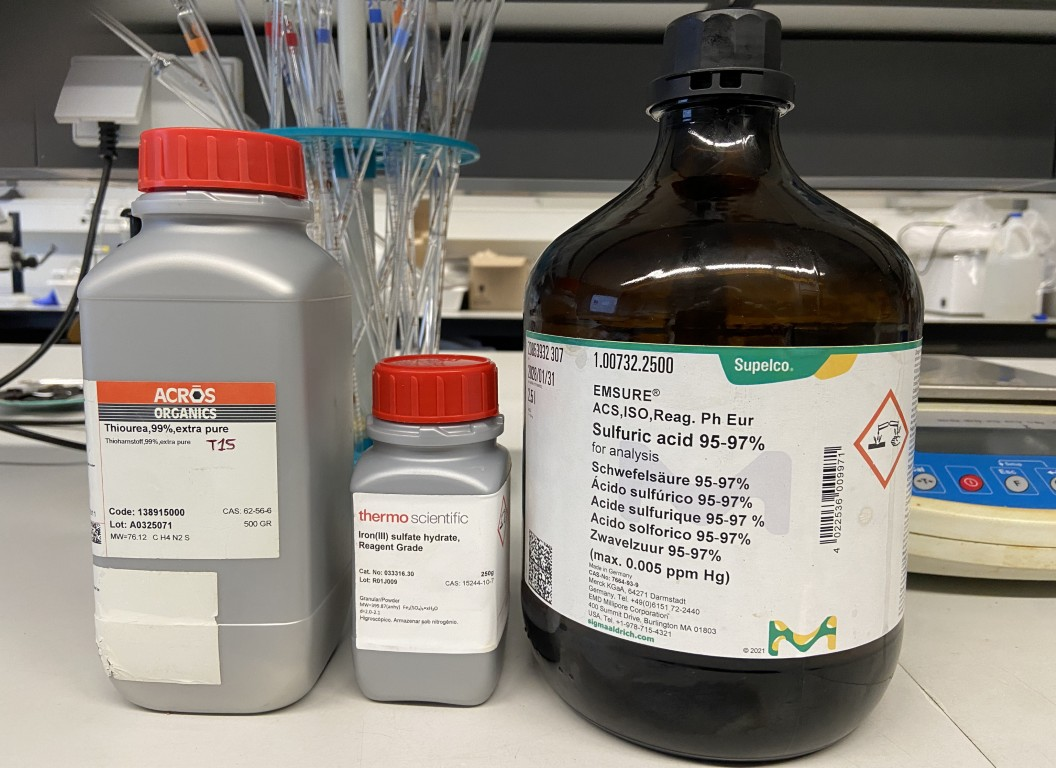
\includegraphics[width=0.9\textwidth]{figures/Reagentes Tioureia.JPG}
    \caption{Reagentes utilizados na lixiviação com Tioureia, ensaio 2.}
    \label{fig:reagentes-tioureia2}
\end{marginfigure}

\begin{itemize}
    \item[-] Tioureia, \tioureia{} - 200~g/kg de minério;
    \item[-] Sulfato de ferro (III) penta-hidratado, \sulfe{}: 0,5~g/kg de minério;
    \item[-] Ácido sulfúrico, \acsul{} - o necessário para obter uma solução com pH = 1.
\end{itemize}

Utilizou-se 100~g de material restante do saco \texttt{A08.4}, para a lixiviação.
Foi utilizada uma relação sólido-líquido de 1 para 5 (S/L = 1/5), portanto para 100~g de sólido teremos 500~mL de líquido.

A lixiviação foi efetuada a uma temperatura ambiente, com uma agitação de 350~rpm, durante 6~horas.
Foi utilizado um reator de borossilicato de 500~mL.

\marginnote{As alterações feitas em relação ao
ensaio preliminar foram a temperatura (de 60~\graus{} para temperatura ambiente), a concentração de tioureia (de 100~g/kg para 200~g/kg) e a concentração de sulfato de ferro (III) penta-hidratado (de 0,5~g/kg para 1~g/kg).}

A quantidade de reagentes adicionada foi a seguinte:
\begin{itemize}
    \item[-] $\mathrm{m}_{\left[\tioureia{}\right]}$ = 20~g;
    \item[-] $\mathrm{m}_{\left[\sulfe{}\right]}$ = 0,123~g;
    \item[-] $\mathrm{V}_{\left[\acsul{}\right]}$ = 1,7~mL para ajustar pH = 1.
\end{itemize}

No reator de borossilicato, foi adicionado 500~mL de água destilada e 20~g de \tioureia{}. 
Dissolveu-se a \tioureia{} e ajustou-se o pH, adicionando 1,7~mL de \acsul{}, que resultou num pH = 1,251.
Após acidificar a solução, adicionou-se \sulfe{} e o minério no reator, regulando o agitador para 350~rpm e dando início à lixiviação às 10h40.

Após 5~minutos de lixiviação, interrompeu-se a agitação e mediu-se o pH (1,315). 
Foi-se verificando o pH ao longo da lixiviação, para garantir que a solução se encontrava com pH = 1, adicionando \acsul{} sempre que necessário.

Adicionou-se, durante as 6~horas de lixiviação, 0,6~mL de \acsul{}. No total, adicionou-se 2,3~mL de \acsul{}, sendo que 1,7~mL foram adicionados antes da lixiviação e 0,6~mL durante a lixiviação para manter o pH = 1.

Foi preparada uma solução de lavagem com água destilada acidificada (pH = 1,099). 
A relação S/L para lavagem foi de 1/1,5, ou seja, 150~mL de solução de lavagem para 100~g de minério.

Uma vez terminada a lixiviação, filtrou-se a o material com um sistema de filtragem composto por um filtro de Büchner, um balão Kitasato, papel de filtro e bomba de vácuo.
Filtrou-se a solução, mediu-se o volume de licor filtrado (495~mL) e mediu-se o pH do licor (1,801).

\begin{marginfigure}
    \centering
    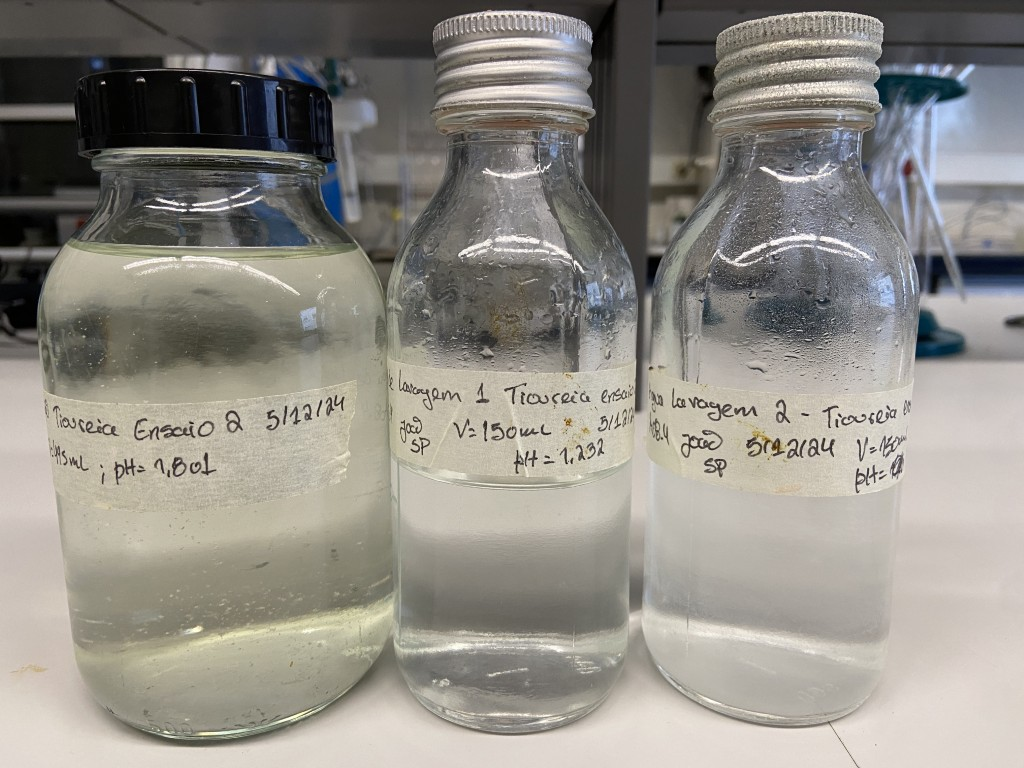
\includegraphics[width=0.9\textwidth]{figures/Licores de lixiviação - tioureia ensaio 2}
    \caption{Licor de lixiviação e águas de lavagem da lixiviação com Tioureia, ensaio 2.}
    \label{fig:licores-lixiviacao-tioureia-ensaio2}
\end{marginfigure}

Irão ser efetuadas duas lavagens, portanto colocou-se o sólido filtrado novamente no reator de borossilicato e adicionou-se 150~mL de solução de lavagem.
Deixou-se a lavar durante 30~minutos, com agitação de 350~rpm.
Uma vez terminada a lavagem, filtrou-se novamente com o mesmo sistema de filtragem.
Mediu-se o volume da água de lavagem (150~mL) e mediu-se o pH da água de lavagem (pH = 1,232).

\marginnote{Ocorreu novamente precipitação de sólido nos frascos de armazenamento do licor de lixiviação e das águas de lavagem. Ver Figura~\ref{fig:precipitado-lix-tioureia}.}

Colocou-se o sólido filtrado novamente no reator de borossilicato e adicionou-se 150~mL de solução de lavagem, para efetuar a segunda lavagem.
Deixou-se a lavar durante 30~minutos, com agitação de 350~rpm.
Uma vez terminada a lavagem, filtrou-se novamente com o mesmo sistema de filtragem.
Mediu-se o volume da água de lavagem (150~mL) e mediu-se o pH da água de lavagem (pH = 1,216).

% \begin{marginfigure}
%     \centering
%     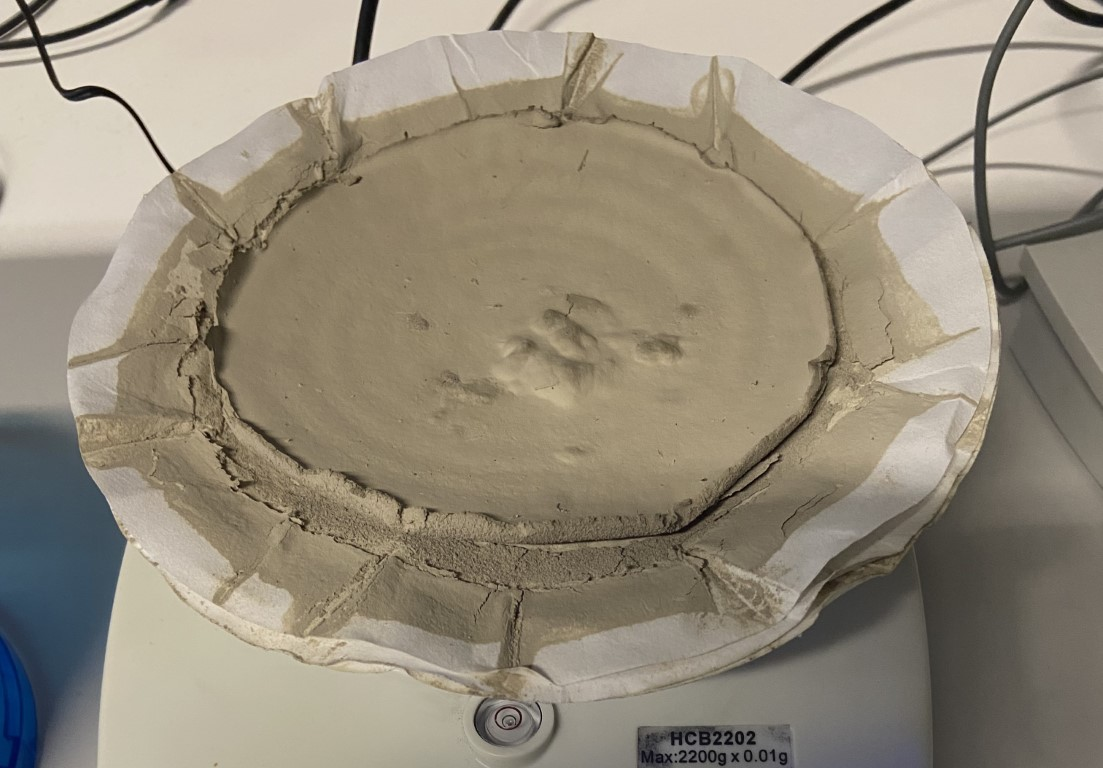
\includegraphics[width=0.9\linewidth]{figures/Resíduo Sólido Lixiviação Tioureia Ensaio 2.jpg}
%     \caption{Resíduo sólido seco da lixiviação com Tioureia, ensaio 2.}
%     \label{fig:residuo-solido-tioureia-ensaio2}
% \end{marginfigure}

Tanto o licor de lixiviação como as águas de lavagem foram guardados em frascos devidamente identificados para posterior análise.

O sólido filtrado foi colocado numa placa de Petri e deixado a secar na estufa a 60~\graus{} durante 10~horas.

\begin{marginfigure}[\baselineskip]
    \centering
    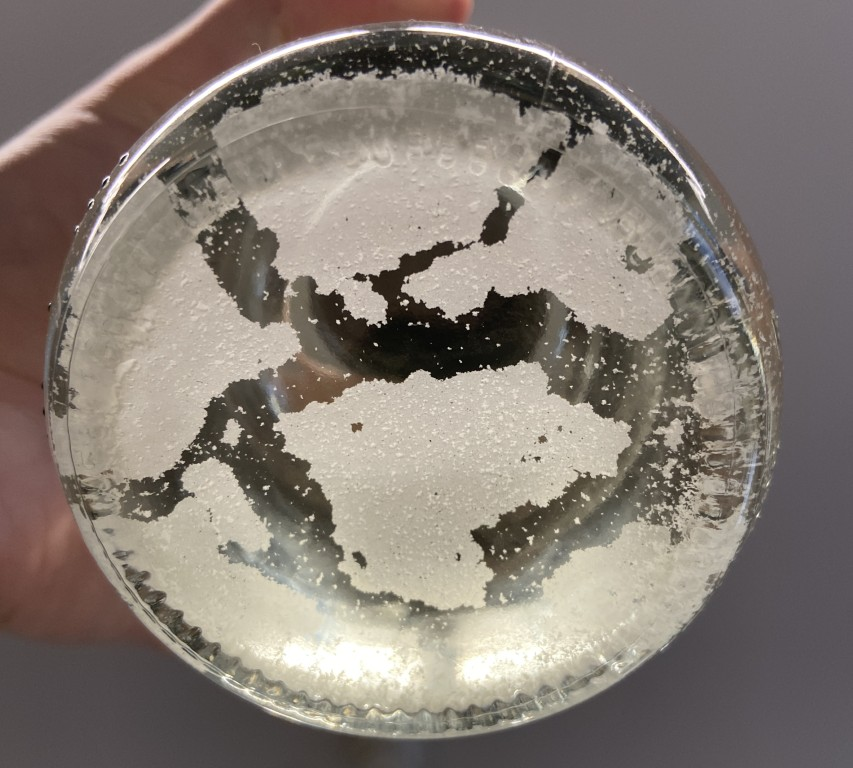
\includegraphics[width=0.9\textwidth]{figures/Precipitado Toureia}
    \caption{Precipitado no licor de lixiviação com Tioureia, ensaio 2.}
    \label{fig:precipitado-lix-tioureia}
\end{marginfigure}

Após estar seco, mediu-se a massa do resíduo de lixiviação, subtraindo as massas dos papéis de filtro - 89,49~g.

O resíduo sólido será submetido a digestão ácida para análise posterior na absorção atómica.

\newthought{Concentrações em \ce{Au}:} Licor de lixiviação - 1,088~mg/L; Água de lavagem 1 - 0,64~mg/L; Água de lavagem 2 - 0,13~mg/L; resíduo (média) - 6,90~ppm.

\hrulefill

\newday{Digestões ácidas dos resíduos de lixiviação - Tioureia, ensaio 2}

Hoje realizou-se as digestões ácidas do resíduo sólido proveniente da lixiviação com Tioureia, ensaio 2, do dia~\nameref{day:4-dezembro-2024}.

O procedimento seguido para a preparação da amostra para ser colocada na mufla e da digestão ácida em si foi os do dia~\nameref{day:7-novembro-2024} e \nameref{day:8-novembro-2024}, respetivamente.

Após a análise na absorção atómica, obteve-se a Tabela~\ref{tab:aas-concentracao-au-res-tioureia2} referente às concentrações em \ce{Au} no resíduo de lixiviação com Tioureia, ensaio 2.

\begin{table}[!ht]
    \centering
    \begin{tabularx}{\textwidth}{@{}lCCC@{}}
        \toprule
        \textbf{Amostra} & \textbf{Absorção} & \textbf{Conc. (mg/L)} & \textbf{Teor \ce{Au} (ppm)} \\ \midrule
        \textbf{Dig. 1} & 0,02813 & 1,01 & 5,0587 \\
        \textbf{Dig. 2} & 0,04310 & 1,54 & 7,7224 \\
        \textbf{Dig. 3} & 0,04126 & 1,48 & 7,3950 \\
        \textbf{Dig. 4} & 0,04119 & 1,48 & 7,3826 \\
        \textbf{Dig. 5} & 0,03875 & 1,39 & 6,9484 \\ \bottomrule
    \end{tabularx}
    \caption{Concentração em \ce{Au} no resíduo de lixiviação com Tioureia, ensaio 2.}
    \label{tab:aas-concentracao-au-res-tioureia2}
\end{table}

Da absorção atómica também se determinou a concentração em \ce{Au} do licor de lixiviação (\textbf{1,088~mg/L}), da água de lavagem 1 (\textbf{0,64~mg/L}) e da água de lavagem 2 (\textbf{0,13~mg/L}).

\hrulefill

\newday{11 Dezembro 2024}

Hoje realizou-se a segunda lixiviação com Citrato de Sódio di-hidratado, \citratodi{}. Utilizou-se o material que sobrou do ensaio preliminar, realizado no dia~\nameref{day:29-novembro-2024}, o saco \texttt{A08.2}.

Utilizou-se os mesmos reagentes: citrato de sódio di-hidratado, \citratodi{}; tiossulfato de sódio penta-hidratado \tsp{}; sulfato de cobre penta-hidratado, \sulfcu{}; hidróxido de sódio, \hidso{}.
\marginnote{As alterações feitas em relação ao ensaio preliminar foram a concentração do tiossulfato de sódio penta-hidratado (de 0,2~M para 0,1~M) e a temperatura de lixiviação (de 90~\graus{} para 70~\graus{}).}
As concentrações de cada um dos reagentes foi a seguinte:

\begin{itemize}
    \item[-] \citratodi{} = 0,2~M;
    \item[-] \tsp{} = 0,1~M;
    \item[-] \sulfcu{} = 0,1~M;
    \item[-] \hidso{} = 5~M e 15~M.
\end{itemize}

A lixiviação foi realizada com uma relação sólido-líquido de 1 para 5 (S/L = 1/5) e foi utilizado 100~g de minério.

A lixiviação foi efetuada a 90~\graus{}, com uma agitação de 400~rpm, durante 9~horas.

\begin{marginfigure}
    \centering
    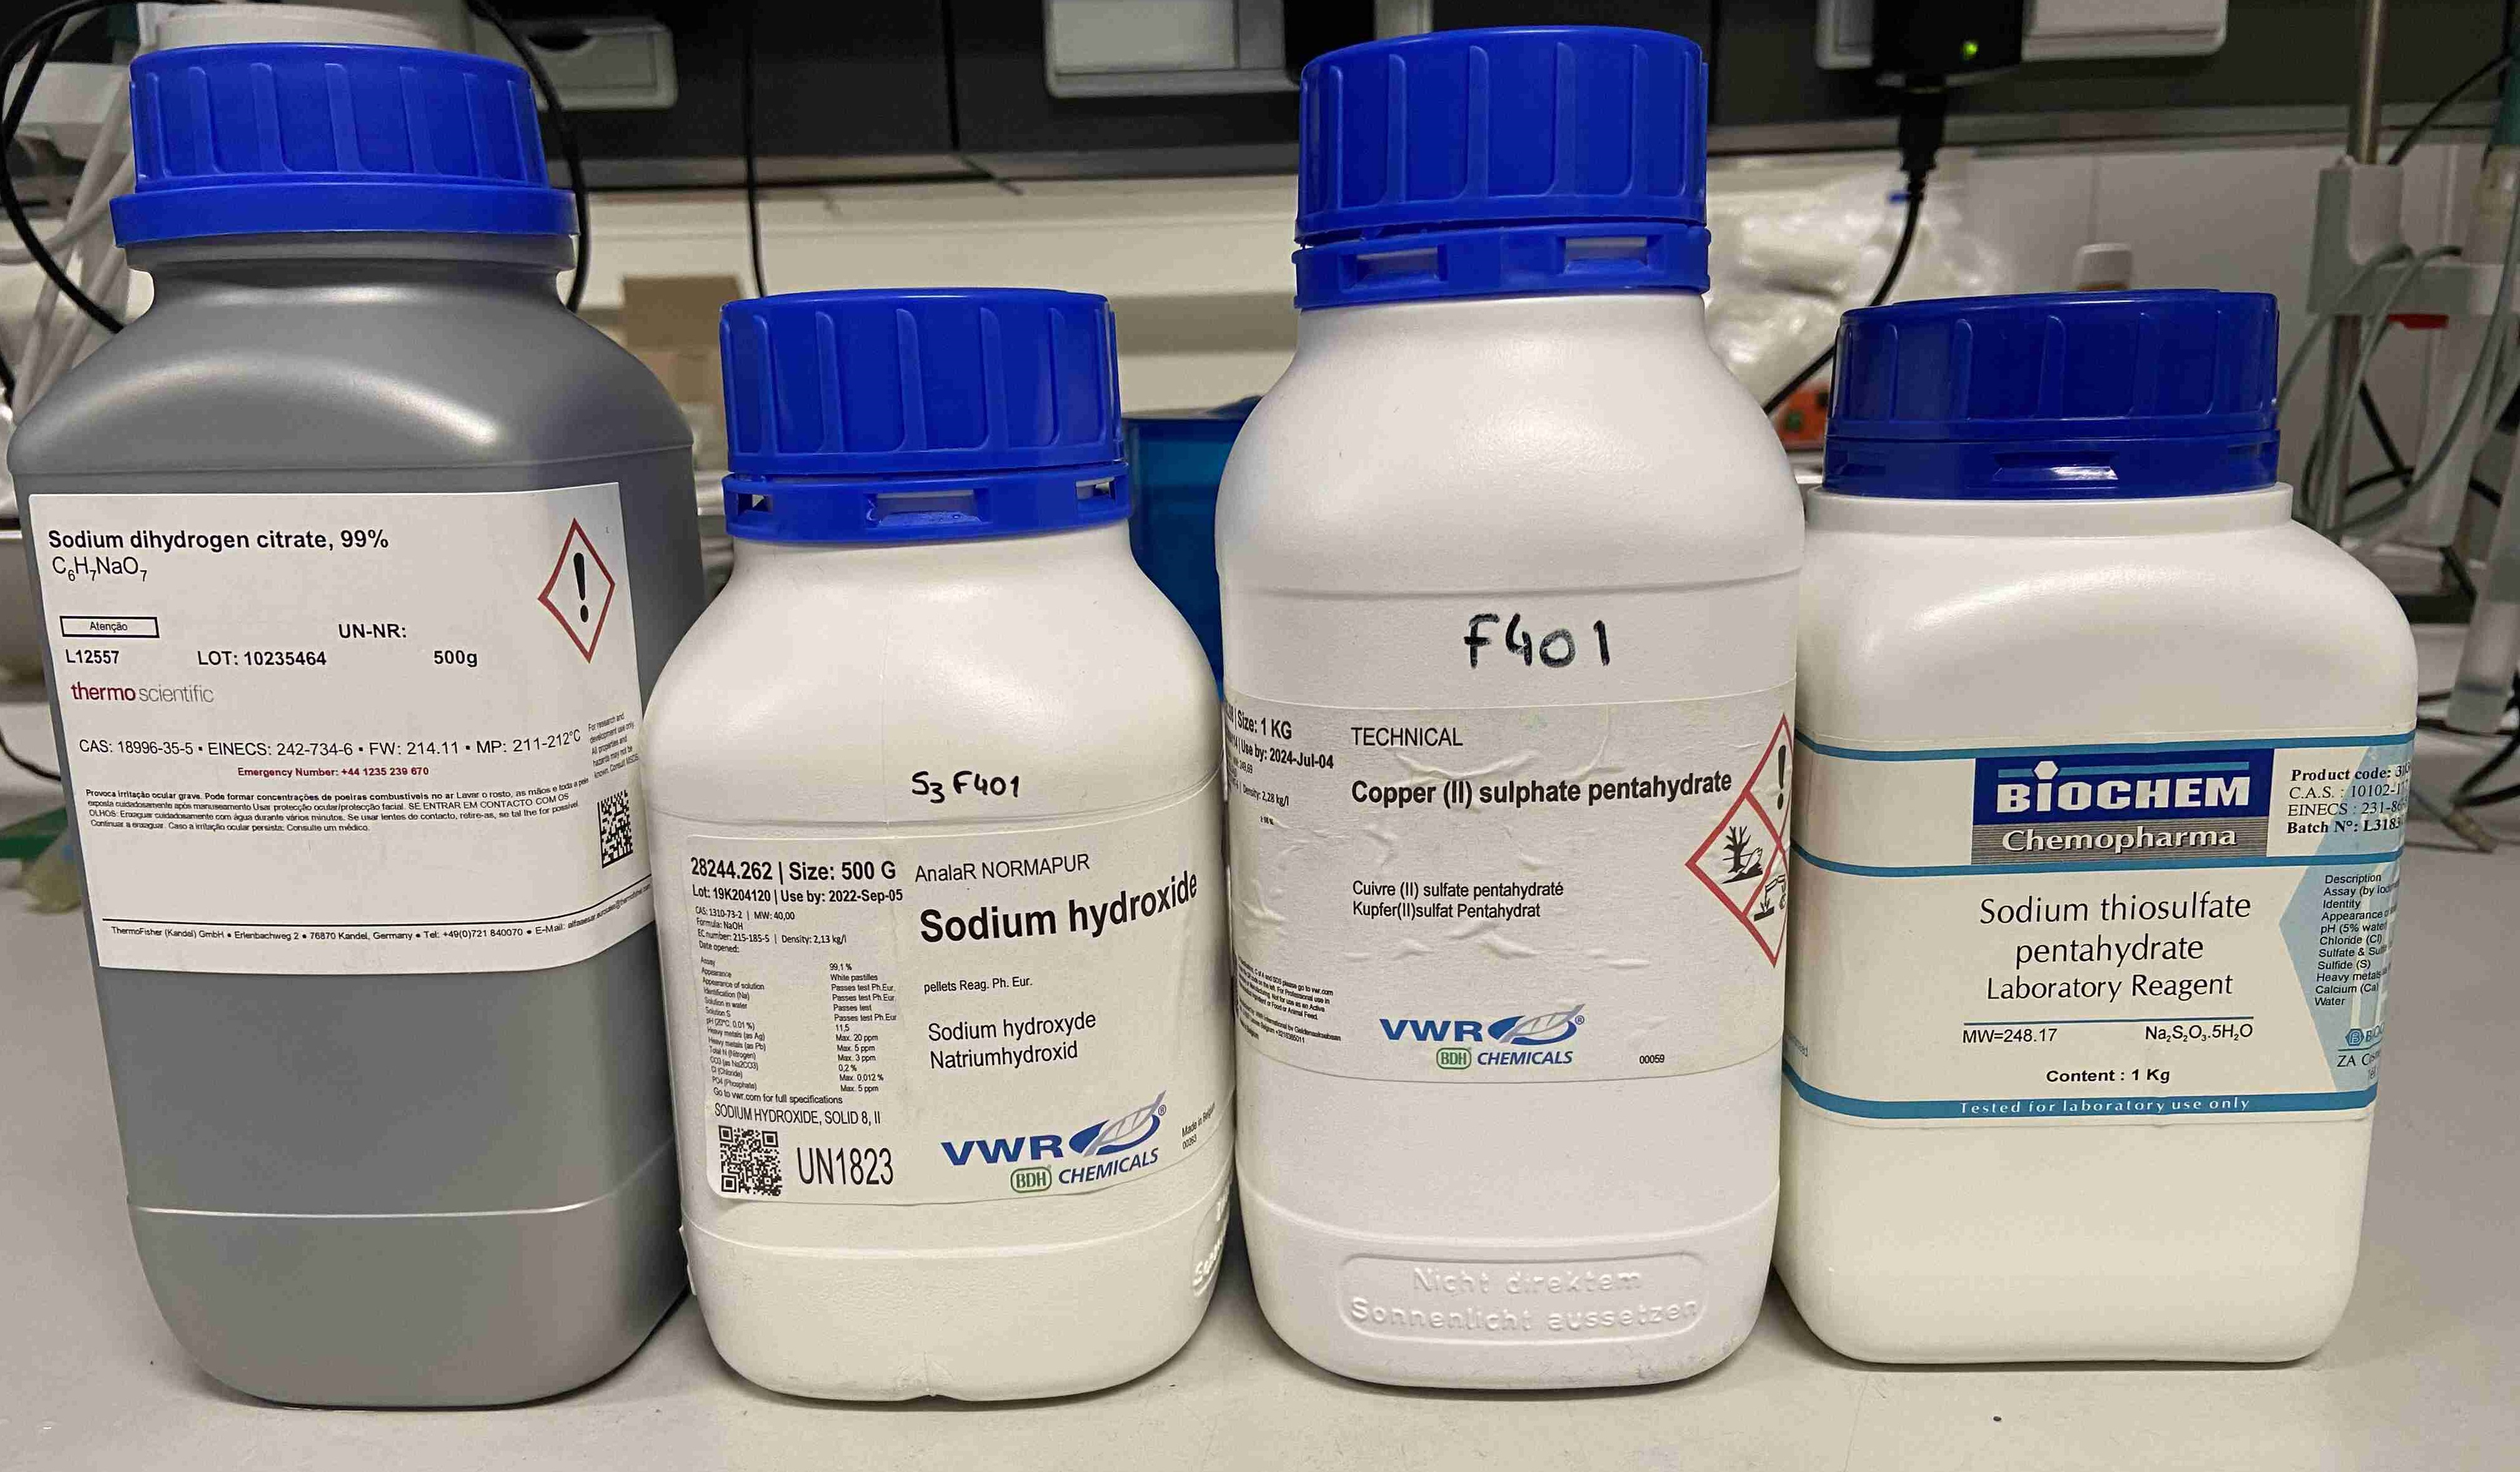
\includegraphics[width=0.9\linewidth]{figures/reagentes lixiviação citrato}
    \caption{Reagentes utilizados na segunda lixiviação (citrato).}
    \label{fig:reagentes-lix-citrato2}
\end{marginfigure}

As quantidades de reagentes adicionadas foram as seguintes:

\begin{itemize}
    \item[-] $\mathrm{m}_{\left[\citratodi{}\right]}$ = 21,41~g;
    \item[-] $\mathrm{m}_{\left[\tsp{}\right]}$ = 12,41~g;
    \item[-] $\mathrm{m}_{\left[\sulfcu{}\right]}$ = 12,48~g.
\end{itemize}

Num gobelé, foi medida a massa de citrato de sódio di-hidratado (21,41~g), a massa de tiossulfato de sódio penta-hidratado (12,41~g) e a massa de sulfato de cobre penta-hidratado (12,48) que vão ser utilizados.
Num balão volumétrico de 500~mL foi medido o volume de água necessário para respeitar a relação sólido-líquido.

Colocou-se, no reator de borossilicato, os 500~mL de água destilada e juntou-se os reagentes sólidos.
Colocou-se o agitador mecânico, regulado a 400~rpm e dissolveu-se os reagentes na água destilada, antes de se colocar o minério.

Mediu-se o pH da solução de lixiviação, sem o minério (pH = 2,895).
Adicionou-se uma solução\sidenote{Na verdade, foram adicionadas duas soluções com diferentes concentrações. Primeiramente uma solução de \hidso{} a 5~M, mas como o pH continuava fora do intervalo desejado após se adicionar uma quantidade considerável, trocou-se para uma solução a 15~M, para prevenir alterações na relação sólido-líquido.} de \hidso{}, para que o pH da solução de lixiviação estivesse dentro do intervalo [7; 11].
O pH medido da solução de lixiviação sem o minério, após a adição de 3,4~mL de \hidso{} a 5~M e 2,15~mL de \hidso{} a 15~M, foi de 11,85.

Uma vez ajustado o pH, adicionou-se as 100~g de minério à solução de lixiviação e deu-se início à lixiviação, pelas 10h30.
Deixou-se lixiviar durante 5~minutos e mediu-se novamente o pH (5,8).
Ajustou-se novamente o pH, pela adição 1,85~mL de \hidso{} a 15~M, até que o pH fosse de 7,246.

Foi-se medindo o pH de hora em hora. 
O valor de pH manteve-se constante, pelo que não foi necessário adicionar mais \hidso{} durante a lixiviação.

No fim das 9~horas de lixiviação, filtrou-se a solução com um sistema de filtragem composto por um filtro de Büchner, um balão Kitasato, papel de filtro e bomba de vácuo.
Filtrou-se e mediu-se o volume de licor de lixiviação (487~mL). 
Mediu-se o pH (6,719) e guardou-se o licor de lixiviação num frasco devidamente identificado.

O bolo de minério foi lavado com 150~mL de água destilada. 
Foi utilizada uma relação de lavagem de 1 para 1,5 (S/L = 1/1,5) e efetuaram-se duas lavagens, de 30~minutos cada.

Após a primeira lavagem, filtrou-se o material e mediu-se o volume da água da 1ª lavagem (112~mL) e o pH (pH = 6,970) \sidenote{O volume de água de lavagem filtrada é muito inferior aos 150~mL de água de lavagem adicionada, porque o filtro de papel colmatou e não se conseguiu filtrar os 38~mL de água restante. Colocou-se o bolo com a água de novo no reator e procedeu-se à segunda lavagem, adicionando na mesma os 150~mL de água destilada.}.
O volume de água filtrada da 2ª lavagem foi de 156~mL e o pH medido foi de 7,676.
As águas de lavagem foram devidamente identificadas e colocadas em recipientes de vidro.

O material, já lavado e filtrado, foi colocado numa placa de Petri e deixado a secar na estufa a 60~\graus{} durante 10~horas.

Após estar seco, mediu-se a massa do resíduo de lixiviação, subtraindo as massas dos papéis de filtro - 90,29~g.

O resíduo sólido seco foi desagrado no moinho de anéis, e colocado na mufla para se proceder à digestão ácida.

\newthought{Concentrações em \ce{Au}:} Licor de lixiviação - 1,34~mg/L; Água de lavagem 1 - 0,31~mg/L; Água de lavagem 2 - 0,30~mg/L; resíduo (média) - 6,67~ppm.

\hrulefill

\newday{Digestões ácidas dos resíduos de lixiviação - Citrato, ensaio 2}

Realizou-se a digestão ácida do resíduo sólido proveniente da lixiviação com citrato de sódio di-hidratado, ensaio 2, do dia~\nameref{day:11-dezembro-2024}.
O procedimento seguido foi o mesmo que o do dia~\nameref{day:7-novembro-2024} e \nameref{day:8-novembro-2024}.

Após a digestão ácida, procedeu-se à análise na absorção atómica.
Após essa análise, obteve-se a Tabela~\ref{tab:aas-concentracao-au-res-citrato2} referente às concentrações em \ce{Au} no resíduo de lixiviação com citrato de sódio di-hidratado, ensaio 2.

\newpage

\begin{table}[!ht]
    \centering
    \begin{tabularx}{\textwidth}{@{}lCCC@{}}
        \toprule
        \textbf{Amostra} & \textbf{Absorção} & \textbf{Conc. (mg/L)} & \textbf{Teor \ce{Au} (ppm)} \\ \midrule
        \textbf{Dig. 1} & 0,04577 & 1,32 & 6,5853 \\
        \textbf{Dig. 2} & 0,04538 & 1,31 & 6,5289 \\
        \textbf{Dig. 3} & 0,04684 & 1,35 & 6,7399 \\
        \textbf{Dig. 4} & 0,04634 & 1,33 & 6,6676 \\
        \textbf{Dig. 5} & 0,04762 & 1,37 & 6,8526 \\ \bottomrule
    \end{tabularx}
    \caption{Concentração em \ce{Au} no resíduo de lixiviação com Citrato, ensaio 2.}
    \label{tab:aas-concentracao-au-res-citrato2}
\end{table}

Da absorção atómica também se determinou a concentração em \ce{Au} do licor de lixiviação (\textbf{1,34~mg/L}), da água de lavagem 1 (\textbf{0,31~mg/L}) e da água de lavagem 2 (\textbf{0,30~mg/L}).

\hrulefill

% \newday{9 Janeiro 2025}

% Hoje realizou-se a segunda lixiviação com Tiossulfato
% \section{Resultados da Segunda Etapa de Lixiviações}

% \subsection{Tioureia, ensaio 2}